\documentclass[a4paper,12pt,twoside]{book}

\usepackage{pacchetti}																%PACCHETTI USATI
\usepackage{macro}																		%MACRO IMPLEMENTATE
\makeindex																						%CREA INDICE ANALITICO

\begin{document}  
	\title{Accoppiamento con vincoli di risorsa}				%CREA TITOLO
	\author{Andrea Gardoni \hfill xxxxxx}
	\date{31 Aprile 2007}
	\titolocorso{Progettazione e analisi di algoritmi}
	\degreeyear{2006/2007}															% ANNO ACCADEMICO 
	\principaladviser{Roberto Cordone\hfill}						% RELATORE PRINCIPALE
	
	\maketitle
	\salvastmpB	
	\clearpage{\pagestyle{empty}\cleardoublepage}
	\tableofcontents
	\salvastmpB	
	\clearpage{\pagestyle{empty}\cleardoublepage}
\chapter*{Introduzione}\label{Chap:Intro}
\markboth{Introduzione}{Introduzione}
\addcontentsline{toc}{chapter}{Introduzione}
Il problema affrontato � quello dell'accoppiamento a costo minimo con vincoli di risorsa.\\
Si devono assegnare un certo numero di persone (o macchine o entit�) a un certo numero di progetti (o lavori), in modo che ciascuna sia assegnata a un progetto diverso. Assegnare una persona a un progetto comporta un costo, ma anche l'uso di una risorsa. Si vuole minimizzare il costo totale di tutti gli assegnamenti, garantendo che l'uso totale della risorsa non superi una data disponibilit� (Budget).\\
Un'applicazione pratica del problema pu� essere appunto l'assegnamento di lavoratori a progetti.\\
La tecnica utilizzata per raggiungere la soluzione del problema � di tipo branch and bound. \cite{SCAP}.
	\salvastmpB	
	\clearpage{\pagestyle{empty}\cleardoublepage}
\chapter{Il problema}\label{Chap:Prob}

\section{Definizione}

Il problema affrontato � l'accoppiamento a costo minimo con vincoli di risorsa.

Si devono assegnare $n$ persone (o macchine o entit�) a $n$ progetti (o lavori), in modo che ciascuna persona sia assegnata a un progetto diverso. Assegnare la persona $i$ al progetto $j$ comporta un costo $c_{ij}$, ma anche l'uso di una risorsa in quantit� limitata $r_{ij}$.

Il problema pu� essere definito tramite un grafo bipartito $G=(V_{1} \cup V_{2},E)$ dove il sottoinsieme di vertici $V_{1}$ rappresenta l'insieme delle persone, il sottoinsieme di vertici $V_{2}$ rappresenta l'insieme dei progetti, mentre l'insieme dei lati $E$ rappresenta gli accoppiamenti possibili tra persone e progetti.\\
Si vuole minimizzare il costo totale di tutti gli assegnamenti, garantendo che l'uso totale della risorsa non superi una data disponibilit� $B$ (\emph{Budget}).

\section{Formulazione}

\textsc{Dati}:
\begin{itemize}
	\item $|V_{1}|=n$ persone e $|V_{2}|=n$ progetti
	\item $c_{ij}$ costo di attribuzione progetto $j \in V_{2}$ alla persona $i \in V_{1}$
	\item $r_{ij}$ risorsa consumata dalla persona $i \in V_{1}$ per il fare il progetto $j \in V_{2}$
		%3)
	\item L'uso di risorse totale:\hfill
		\begin{equation}
			R = \displaystyle\sum_{i \in V_{1}}\ds\sum_{j \in V_{2}} r_{ij}
		\end{equation}
	%4)
	\item Il budget $B$, viene calcolato come ($\rho$ � un parametro):\hfill
		\begin{equation}\label{eq:budget_cal}
			B = \displaystyle\frac{R}{n} \cdot \rho \qquad \rho \in \left\{ 0.6,0.8,0.1 \right\}
		\end{equation}
\end{itemize}
\textsc{Variabili}:
	\begin{itemize}
		\item Una soluzione � individuata dalle variabili:
	\end{itemize}
	\begin{equation*}
		x_{i,j}=
			\begin{cases}		
				1& \text{progetto $j \in V_{2}$ alla persona $i \in V_{1}$},\\		
				0& \text{altrimenti}.
			\end{cases}
	\end{equation*}
\textsc{Vincoli}:
\begin{itemize}
	%1)
	\item Una persona deve essere associata a un solo progetto:\hfill
		\begin{equation}\label{eq:prog_lav0}
			\displaystyle\sum_{j \in V_{2}}x_{ij}=1 \qquad i \in V_{1}
		\end{equation}
	%2)
	\item Un progetto deve essere associato a una sola persona:\hfill
		\begin{equation}\label{eq:lav_prog0}
			\displaystyle\sum_{i \in V_{1}}x_{ij}=1\qquad j \in V_{2}
		\end{equation}
	%3)
	\item Vincolo di budget\hfill
		\begin{equation}\label{eq:budget0}
			\ds\sum_{i \in V_{1}}\ds\sum_{j \in V_{2}} r_{ij} x_{ij} \leq B
		\end{equation}
\end{itemize}
\textsc{Obiettivo}:
\begin{itemize}
	\item Si vuole minimizzare il costo totale:
		\begin{equation}
			\min\ \ds\sum_{i \in V_{1}}\ds\sum_{j \in V_{2}} c_{ij} x_{ij} 
		\end{equation}
\end{itemize}

	\clearpage{\pagestyle{empty}\cleardoublepage}
\chapter{L'algoritmo di minimizzazione}\label{Chap:Algo}
Per la risoluzione del problema utilizziamo la tecnica del Branch and Bound, la quale si basa sulla scomposizione del problema originale in sottoproblemi (nodi), pi� semplici da risolvere.\\
Per limitare il numero di nodi da esaminare si associa ad ogni nodo un ``lower bound'', ossia un limite inferiore, che indica una stima per difetto del valore di tutte le soluzioni complete ottenibili come discendenti di quel nodo. Anche un ``upper bound'' deve essere noto e viene usato come termine di confronto per i lower bounds dei nodi. L'upper bound � il valore della migliore soluzione trovata sinora. Se un nodo dell'albero ha un lower bound maggiore o uguale all'upper bound corrente, esso viene chiuso, cio� viene eliminato dalla lista dei nodi aperti. Infatti tutte le soluzioni complete che si otterrebbero da esso avrebbero un valore non migliore del valore della soluzione ottima corrente. La stessa cosa avviene se si dimostra che il consumo di risorsa sul nodo non pu� essere inferiore al budget perch� le soluzioni complete che sottrarrebbero non possono essere ammissibili .

\section{Calcolo del lower bound}

Per il calcolo del lower bound (\verb|LB|), una prima idea � quella di ignorare il vincolo del $Budget$ affinch� il problema diventi risolvibile in tempo polinomiale $O(N^{3})$, dato che si riduce a un linear assignement problem. Questo pu� essere risolto usando l'algoritmo descritto in \cite{shortLap}, disponibile in rete come libreria \verb|lap.c|.\\
Il linear assignement problem, � definito come segue:\\
\textsc{Dati}:
\begin{itemize}
	\item $|V_{1}|=n$ persone e $|V_{2}|=n$ compiti
	\item $c_{ij}$ costo di attribuzione del compito $j \in V_{2}$ alla persona $i \in V_{1}$
\end{itemize}
\textsc{Variabili}:
	\begin{equation*}
		x_{i,j}=
			\begin{cases}		
				1& \text{compito $j \in V_{2}$ a persona $i \in V_{1}$},\\		
				0& \text{altrimenti}.
			\end{cases}
	\end{equation*}
\textsc{Vincoli}:
\begin{itemize}
	%1)
	\item Una persona deve essere associata a un solo progetto:\hfill
		\begin{equation}\label{eq:prog_lav}
			\displaystyle\sum_{j \in V_{2}}x_{ij}=1 \qquad i \in V_{1}
		\end{equation}
	%2)
	\item Un progetto deve essere associato a una sola persona:\hfill
		\begin{equation}\label{eq:lav_prog}
			\displaystyle\sum_{i \in V_{1}}x_{ij}=1\qquad j \in V_{2}
		\end{equation}
	%3)
	\item Vincolo di budget\hfill
		\begin{equation}\label{eq:budget}
			\ds\sum_{i \in V_{1}}\ds\sum_{j \in V_{2}} r_{ij} x_{ij} \leq B
		\end{equation}
\end{itemize}
\textsc{Obiettivo}:
\begin{itemize}
	\item si vuole minimizzare il costo totale:
		\begin{equation}
			\min\ \ds\sum_{i \in V_{1}}\ds\sum_{j \in V_{2}} c_{ij} x_{ij} 
		\end{equation}
\end{itemize}
Il calcolo del lower bound, avviene nella funzione \verb|ProcessBnode| da parte della funzione \verb|CalcoloLB|, che riceve: il nodo corrente \verb|N|, i dati del problema \verb|PD|, e la soluzione migliore (Best Solution) \verb|BS|.
Nella struttura dati del nodo, \verb|N.LB|, viene salvato il valore del lower bound calcolato tramite la funzione \verb|lap|, la quale riceve come input la dimensione del problema, \verb|dim| e la matrice dei costi \verb|assigncost|, e fornisce come output la soluzione stessa, descritta attraverso i due vettori \verb|LBcolsol| e \verb|LBrowsol| che riportano, rispettivamente, la persona a cui � assegnato ogni progetto e il progetto assegnato a ogni persona.

\section{Penalit� Lagrangiane}\label{sec:Penalit�Lagrangiane}

Per evitare di generare tramite branching nodi che non possono portare un miglioramento, vengono inserite condizioni note come penalit� lagrangiane. Se il costo ridotto di una cella della matrice dei costi, � maggiore dell'intervallo esistente tra l'upper bound e il lower bound, allora � possibile scartare tale cella fissando la corrispondente cella nella matrice dei vincoli a zero. Questo perch� tale costo stima per difetto l'incremento che la funzione obiettivo subirebbe forzando la corrispondente variabile a 1.

%==========================================================================
%		Secondo lower bound Zaino a scelta multipla, tolto in un secondo momento non controllato!
%==========================================================================
%\section{Calcolo del secondo lower bound}
%Nel calcolo del primo lower bound abbiamo trascurato il vincolo del budget (cfr. (\ref{eq:budget}) a Pagina \pageref{eq:budget}), mentre per il calcolo del secondo, abbiamo trascurato il vincolo che associa a ogni persona a un solo progetto (cfr. (\ref{eq:lav_prog}) a Pagina \pageref{eq:lav_prog}).\\
%In questo modo, si ottiene il problema dello zaino a scelta multipla, risolvibile con la procedura: \verb|fmcknap.c|. \cite{caselli,Pis95Mcknap}\\
%%Il codice \verb|fmcknap.c|, risolve il problema della massimizzazione, di conseguenza il nostro problema deve essere descritto come:
%Il problema dello zaino a scelta multipla � definito come:\\
%\textsc{Variabili}:
%	\begin{itemize}
%		\item $x_{ij}\in \left\{ 0,1\right\}$
%	\end{itemize}
%\textsc{Vincoli}:
%	\begin{itemize}
%		\item $\ds\sum_{j} x_{ij}=1 \qquad \forall_{i}$
%		\item $\ds\sum_{ij} r_{ij}x_{ij} \leq B$
%	\end{itemize}
%\textsc{Obiettivo}:
%	\begin{itemize}
%		\item  $\ds\sum_{ij} a_{ij}x_{ij}$
%	\end{itemize}
%Per ottenere un'istanza del problema dello zaino a scelta multipla, servono questi passaggi:
%\begin{itemize}
%	\item $min \ds\sum_{ij} \widetilde{c}_{ij} x_{ij} \quad\Rightarrow\quad - max \ds\sum_{ij} -\widetilde{c}_{ij} x_{ij}$\\
%	Dove $\widetilde{c}_{ij}$, rappresenta la matrice dei costi a cui sono stati sottratti i vettori $u_{i}$ e $v_{j}$: $\widetilde{c}_{ij}= c_{ij}-u_{i}-v_{j}$.
%	\item trovo il minimo della matrice definito come: $K = -min\ -\widetilde{c}_{ij}$
%	\item sommo il valore $-K$ a tutti i valori della matrice $\widetilde{c}_{ij}$
%	\item pongo $a_{ij}=\widetilde{c}_{ij} - K$
%\end{itemize}
%===========================================================
%		Fine mcknap
%===========================================================
\section{Calcolo dell'upper bound}

Per il calcolo dell'upper bound (\verb|UB|), viene creata una nuova matrice $\gamma$~(\verb|gamma|) che contiene una combinazione convessa dei costi e del consumo di risorsa. Essa � quindi definita come $\gamma_{ij}=\alpha \cdot c_{ij}+\left(1-\alpha \right)\cdot r_{ij}$; dove $c_{ij}$ � la matrice dei costi, mentre $r_{ij}$ quella delle risorse. Sulla matrice $\gamma$, viene eseguita la funzione \verb|lap|, la quale restituisce il vettore delle soluzioni \verb|rowsolGamma|; grazie alle coordinate fornite dal vettore, viene calcolato il costo sulla matrice dei costi, e il consumo sulla matrice delle risorse.
\begin{center}
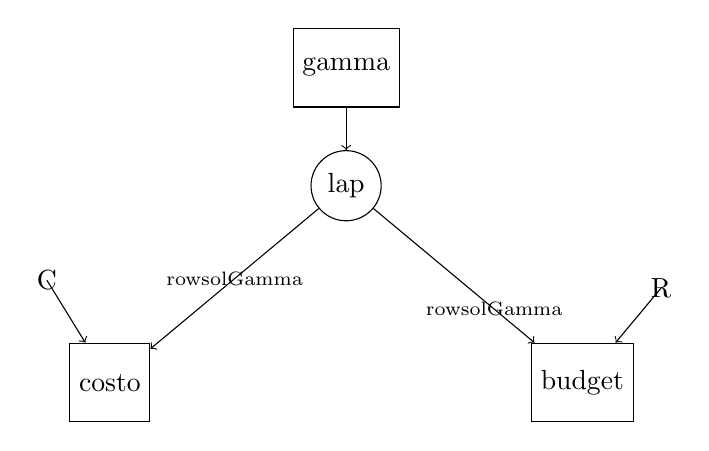
\begin{tikzpicture}
% Nodo Gamma
\draw(0,0)node[minimum height=1cm, minimum width=1cm,draw](node gamma){gamma}
		 % Nodo lap
		 (0,-1.5)node[minimum height=0.5cm, minimum width=0.5cm,draw,circle](node lap){lap}
		 % Nodo matrice costi
		 (-3,-4)node[minimum height=1cm, minimum width=1cm,draw](node cost){costo}
		 % Nodo matrice risorse
		 (+3,-4)node[minimum height=1cm, minimum width=1cm,draw](node bud){budget};

\draw[->](node gamma)--(node lap);
% Freccia da lap a costi
\draw[->](node lap)--(node cost)node[midway]{\scriptsize{rowsolGamma}};
% Matrice costi c freccia piccola
\draw[->](-3.8,-2.7)--(node cost)node[at start]{C};
% Freccia da lap a budget
\draw[->](node lap)--(node bud)node[near end]{\scriptsize{rowsolGamma}};
% Freccia matrice risorse piccola
\draw[->](4,-2.8)--(node bud)node[at start]{R};
\end{tikzpicture}
\end{center}

A ogni iterazione, il suo costo (\verb|UB|), viene confrontato con l'upper bound globale nella struttura dati \verb|BestSolution|, se � minore, viene aggiornata la migliore soluzione trovata fino a quel momento.\\

Infine $\alpha$ � un parametro che varia tra 0 e 1. Valutata (sempre con \verb|lap.c|) la soluzione ottima rispetto a gamma, si pu� calcolarne il consumo totale di risorsa e il costo. Se il consumo � minore o uguale al budget, questo significa che si � dato troppo peso al consumo di risorsa. Quindi il parametro $\al$ cresce come segue:
\begin{align*}
	\al_{m} &= \al\\
	\al_{M} &= \al_{M}\\
	\al     &= \ds\frac{1}{2}\al+\frac{1}{2}\al_{M}.
\end{align*}
Se il consumo � maggiore del budget, questo significa che si � dato troppo poco peso al consumo di risorsa. Quindi il parametro $\alpha$ si modifica come segue:
\begin{align*}
	\al_{M} &= \al\\
	\al_{m} &= \al_{m}\\
	\al     &= \ds\frac{1}{2}\al+\frac{1}{2}\al_{m}.
\end{align*}
L'aggiornamento di $\al$ viene eseguito per 10 iterazioni. Il valore iniziale di $\al$ � 1 (cio� si minimizza il solo consumo di risorsa). Se la soluzione corrispondente ha un consumo superiore al budget B, possiamo concludere che nessuna soluzione del nodo corrente � ammissibile, quindi il nodo si pu� chiudere senza altre elaborazioni.\\
In Pseudocodice \ref{UB} viene mostrata la logica del calcolo.
%Sulla matrice $\gamma$, viene eseguita la funzione \verb|lap|, la quale restituisce il vettore delle soluzioni \verb|rowsolGamma|; grazie alle coordinate fornite dal vettore, viene calcolato il costo sulla matrice dei costi, e il consumo sulla matrice delle risorse.
%\begin{center}
%\begin{tikzpicture}
%% Nodo Gamma
%\draw(0,0)node[minimum height=1cm, minimum width=1cm,draw](node gamma){gamma}
%		 % Nodo lap
%		 (0,-1.5)node[minimum height=0.5cm, minimum width=0.5cm,draw,circle](node lap){lap}
%		 % Nodo matrice costi
%		 (-3,-4)node[minimum height=1cm, minimum width=1cm,draw](node cost){costo}
%		 % Nodo matrice risorse
%		 (+3,-4)node[minimum height=1cm, minimum width=1cm,draw](node bud){budget};
%
%\draw[->](node gamma)--(node lap);
%% Freccia da lap a costi
%\draw[->](node lap)--(node cost)node[midway]{\scriptsize{rowsolGamma}};
%% Matrice costi c freccia piccola
%\draw[->](-3.8,-2.7)--(node cost)node[at start]{C};
%% Freccia da lap a budget
%\draw[->](node lap)--(node bud)node[near end]{\scriptsize{rowsolGamma}};
%% Freccia matrice risorse piccola
%\draw[->](4,-2.8)--(node bud)node[at start]{R};
%\end{tikzpicture}
%\end{center}
%
%A ogni iterazione, il suo costo (\verb|UB|), viene confrontato con l'upper bound globale nella struttura dati \verb|BestSolution|, se � minore, viene aggiornata la migliore soluzione trovata fino a quel momento.\\
\begin{lstlisting}[caption={Calcolo dell'upper bound},label=UB]
CalcoloUB(Nodo, PD, BS)
{
    alpha = 0.5;
    alpham = 0.0;
    alphaM = 1.0;
   
    for (k=0; k<ITERAZIONI; k++) {
        for (i=0; i<dim; i++)
           for (j=0; j<dim; j++)
              gamma[i][j] = alpha*assigncost[i][j]+(1-alpha)*risorse[i][j];
        
        minimoConsumoRisorse = lap (dim, gamma, rowsolGamma, colsolGamma);

        // Calcolo costi
        costo = 0.0;
        for ( i=0; i<dim; i++ )
                costo += assigncost[i][pta->BNinfo.UBrowsol[i]];
        
				// Calcolo del consumo
        consumo = 0.0;
        for ( i=0; i<dim; i++ )
                consumo += risorse[i][pta->BNinfo.UBrowsol[i]];
                
        if ( consumo <= budget ) {
            alphaTemp = alpha;
            alpha = alpha/2 + alphaM/2;
            alpham = alphaTemp;
            if ( costo<pBS->UB )
                pta->BNinfo.UB = costo;
        }
        else {
            alphaTemp = alpha;
            alpha = alpha/2 + alpham/2;
            alphaM = alphaTemp;
        }    
    }    
}
\end{lstlisting}

\section{Strategia di branching}

La strategia di branching consiste nel fissare una variabile ancora libera a 0 oppure a 1. La variabile viene scelta confrontando la soluzione associata al lower bound e quella associata all'upper bound, cio� i due vettori \verb|LBrowsol| e \verb|UBrowsol|. Se i due bound differiscono, le due soluzioni sono diverse. Si osservano le diversit� e si considera la prima variabile presente nella soluzione dell'upper bound e assente in quella del lower bound. La figura seguente illustra un esempio: le matrici rappresentano le soluzioni associate al lower bound (a sinistra) e all'upper bound (a destra). A destra di ogni matrice compaiono i vettori \verb|LBrowsol| e \verb|UBrowsol| che contengono, per ogni riga, l'indice della colonna in cui compare un 1.
\begin{equation*}\label{eq:mat}
\begin{array}{|c|c|c|c|}
\hline
 	& 1 &  & \\
\hline
 1&   &  & \\
\hline
 	&   &  &1 \\
\hline
 	&   &1 &\\
\hline
\end{array} 
\Leftarrow \verb|LBrowsol| \Rightarrow
\begin{array}{|c|}
\hline
 	2\\
\hline
  1\\
\hline
 	4\\
\hline
 	3\\
\hline
\end{array}
\quad
\begin{array}{|c|c|c|c|}
\hline
 	& 1 &  & \\
\hline
 1&   &  & \\
\hline
 	&   & 1 &\textcolor{red}{X} \\
\hline
 	&   & &1\\
\hline
\end{array} 
\Leftarrow \verb|UBrowsol| \Rightarrow
\begin{array}{|c|}
\hline
 	2\\
\hline
  1\\
\hline
 	3\\
\hline
 	4\\
\hline
\end{array}
\end{equation*}

Una volta definito il punto di branching, la funzione \verb|DeriveBnode| crea due figli, copiando nel figlio le informazioni del problema padre e forzando la variabile di branching a 1 nel primo figlio, a 0 nel secondo.

\begin{lstlisting}[caption={DeriveBnode},label=DBN]
DeriveBnode (father, f, son)
{
    // Copio la matrice dei vincoli da padre in figlio
    for (i=0; i<father->BNinfo.dim; i++)
        for (j=0; j<father->BNinfo.dim; j++)
                son->BNinfo.vincoli[i][j] = father->BNinfo.vincoli[i][j];
    
    // Inserisco le informazioni di branching 
    if ( f==1 ) {
        // Fisso a 0 tutti i valori contenuti nella colonna della cella
        // di branching tranne quello della cella stessa.
        son->BNinfo.vincoli[father->branch.i][father->branch.j] = 1;
        for (i=0; i<father->BNinfo.dim; i++)
            if (i != father->branch.i)
                son->BNinfo.vincoli[i][father->branch.j] = 0;

        // Fisso a 0 tutti i valori contenuti nella riga della cella
        // di branching tranne quello della cella stessa.
        for (j=0; j<father->BNinfo.dim; j++)
            if (j != father->branch.j)
                son->BNinfo.vincoli[father->branch.i][j] = 0;
    }    
    else
        son->BNinfo.vincoli[father->branch.i][father->branch.j] = 0;
}
\end{lstlisting}

\section{Strategia di visita dell'albero}

Le strategie di visita implementate sono tre:
\begin{itemize}
	\item depth first search, ovvero in profondit�
	\item breadth first search, ovvero in ampiezza
	\item best first search
\end{itemize}

\subsection{Depth First Search}\label{sec:DepthFirstSearch}

Questa strategia, inserisce il nodo \verb|N| in cima alla lista \verb|BT| dei nodi aperti.\\
Sviluppa, quindi, l'albero in profondit�, partendo dalla radice ed arrivando fino alle foglie. Ad ogni iterazione l'algoritmo sceglie di esplorare uno tra i nodi figli del nodo appena esplorato. Se questo non ha figli, l'algoritmo passa al nodo di pi� basso livello non ancora esplorato.\\
Quindi si esplora un ramo ancora prima di generare quelli successivi.
Siccome i nodi vengono inseriti sempre dalla cima, per poter ottenere la DFS occorre inserire ogni nuovo nodo in cima alla lista.
\begin{lstlisting}[caption={Depth First Search},label=DFS]
if (VisitStrategy == DEPTH_FIRST)
{
	inslista(N,primolista(BT),BT);
}
\end{lstlisting}

\subsection{Breadth First Search}\label{sec:BreadthFirstSearch}

Questa strategia, inserisce il nodo \verb|N| in coda alla lista \verb|BT| dei nodi aperti.\\
Sviluppa, quindi, l'albero in larghezza, considerando prima tutti i nodi dello stesso livello per poi passare a quelli del livello sottostante.
Si inizia calcolando l'upper bound del nodo radice, generando tutti i suoi figli e calcolando i corrispondenti upper bound. Vengono quindi generati tutti i figli di ogni figlio della radice, e cos� via, esplorando sempre tutti i nodi di un livello prima di passare al livello successivo.

\begin{lstlisting}[caption={Depth First Search},label=BFS]
if (VisitStrategy == BREADTH_FIRST)
{
	inslista(N,succlista(ultimolista(BT),BT),BT);
}
\end{lstlisting}

\subsection{Best First Search}\label{sec:BestFirstSearch}

Questa strategia, mantiene la lista dei problemi aperti ordinata per bound crescente. Quindi inserisce il nuovo nodo prima del primo problema peggiore di esso.\\
Ad ogni iterazione l'algoritmo sceglie di esplorare uno tra i nodi a cui � associato il migliore bound della soluzione ottima.

\begin{lstlisting}[caption={Depth First Search},label=BestFS]
if (VisitStrategy == BEST_FIRST)
{
  pos = primolista(BT);
  while (! finelista(pos, BT) )
  {
      if ( pos->BNinfo.LB > pta->BNinfo.LB )
          break;
      pos = succlista(pos,BT);
  }
  inslista(pta,pos,BT);
}
\end{lstlisting}

	\salvastmpB	
	\clearpage{\pagestyle{empty}\cleardoublepage}
\chapter{I risultati sperimentali}\label{sec:IRisultatiSperimentali}

La macchina utilizzata per le sperimentazioni ha le seguenti caratteristiche:
\begin{itemize}
	\item CPU: Intel Core Duo T2400 $1.87\ GHz$
	\item HD: $160\ GB$ $7200\ rpm$
	\item RAM: $1\ GB$
	\item SO: Microsoft Windows XP [Versione 5.1.2600]
	\item marca/modello: Sony VAIO
\end{itemize}
%Descrizione del tipo di macchina utilizzata per le sperimentazioni, linguaggio, sistema operativo 
%e breve riassunto dei risultati ottenuti.

\section{I dati}
I dati che vengono passati al problema sono: la dimensione \verb|dim|, la matrice dei costi \verb|assigncost|, la matrice delle risorse \verb|risorse|.\\
La dimensione del problema � data dalla dimensione della matrice dei costi la quale viene letta da file (vedi Sezione \ref{sec:lettura_mat}), mentre la matrice delle risorse viene generata a partire da quella dei costi (vedi Sezione \ref{sec:gen_ris}). Affinch� l'istanza del problema possa essere codificata nel linguaggio AMPL, � stato necessario formattare il file in modo conforme. Questo ha consentito di risolvere problemi col risolutore gratuito GLPK e conservare quindi il valore ottimo. Le successive sezioni descrivono i passaggi per ottenere tale formattazione.
 
\subsection{Lettura matrice dei costi}\label{sec:lettura_mat}

Dato un file (vedi Istanza \ref{file_org}) contenente la sola matrice dei costi, l'obiettivo della procedura di codifica � quello di formattare la stessa istanza in linguaggio AMPL (vedi Istanza\ref{file_dest} in Sezione \ref{sec:FormatoDiOutputDelleIstanze}).% inoltre viene aggiunta una matrice delle risorse, negativamente correlata a quella dei costi, e il budget. Nella formattazione originale (vedi Istanza \ref{file_org}):
\renewcommand*\lstlistingname{Istanza} 										%RIDENOMINAZIONE DELLA CAPTION IN Istanza 
\begin{lstlisting}[captionpos={b},caption={File istanza originale},label=file_org]
100
52 89 40 77 89 14 9 77 92 77 52 53 96
96 92 76 33 81 92 84 36 81 47 55 87 35
\end{lstlisting}
Nella riga 1, in Istanza \ref{file_org}, troviamo la dimensione dell'istanza; le successive righe contengono i costi $c_{ij}$. 

\subsection{Generazione della matrice delle risorse}\label{sec:gen_ris}

Per la generazione casuale dei consumi di risorsa $r_{ij}$, si � utilizzata l'equazione (\ref{eq:gen_matrix_risorse}):
\begin{equation}\label{eq:gen_matrix_risorse}
	r_{ij}=min\left( c_{min} + c_{max} - c_{ij} + 10 \cdot \lambda \left(0,10\right), c_{max}\right)
\end{equation}
dove $c_{min}$ e $c_{max}$, sono stati calcolati rispettivamente come il minimo ed il massimo elemento della matrice dei costi $c_{ij}$; infine, $\lambda \left(0,10\right)$ rappresenta un numero casuale intero tra $0$ e $10$ generato utilizzando la libreria \emph{rand.h}; il fattore 10 rappresenta un disturbo alla funzione che ritorna un numero intero casuale. Il minimo ottenuto tra i valori sopra e $c_{rand}$, calcolato come \verb|assigncost[n*ran1(seed)][n*ran1(seed)]| rappresenta il consumo di risorsa. L'obietivo � quello di generare istanze difficili, in cui il consumo di risorsa � negativamente correlato al costo $c_{ij}$; in quanto quelle poco costose tendono a essere inammissibili; e viceversa le ammissibili a essere costose.

\subsection{Formato di output delle istanze}\label{sec:FormatoDiOutputDelleIstanze}

La nuova formattazione � rappresentata in Istanza \ref{file_dest} ordinata per righe crescenti e per colonne crescenti:
\begin{lstlisting}[captionpos={b},caption={File istanza nuovo},label=file_dest]
param N := 100;
param C := 
[0,0] 52 [0,1] 89 [0,2] ...
param R := 
[0,0] 89 [0,1] 94 ...
param B := 75;
end;
\end{lstlisting}
La prima riga riporta la dimensione dell'istanza. Segue la matrice dei costi nel formato $[i,j]$ $c_{ij}$, quindi la matrice delle risorse definita in modo analogo a quella dei costi, infine il budget $B$ e infine il terminatore end.

\newpage
\section{Risultati}

\subsection{Consumi casuali}\label{sec:ConsCasuali}

I risultati mostrati nella Tabella \ref{tab:consCasuali} si riferiscono a istanze del problema in cui sia la matrice dei costi che la matrice delle risorse, sono generate in modo casuale; la matrice delle risorse � comune alle cinque istanze di ciascuna dimensione.\\
La prima colonna contiene il nome dell'istanza; la seconda la dimensione, la terza il budget, la quarta colonna rappresenta il valore migliore ottenuto dal nostro algoritmo, la quinta riporta in secondi il numero di nodi generati, l'ultima colonna il tempo di computazione. Gli ottimi sono stati tutti verificati con GLPK.


\begin{longtable}{|c|c|c|c|c|c|}
\caption{Risultati per le istanze costi risorse casuali}\label{tab:consCasuali}\\
\hline
Nome ist. & Dim. & Budget &Sol. & n� nodi & Tempo\\
\hline
\hline
\endfirsthead
\hline
Nome ist. & Dim. & Budget &Sol. &  n� nodi & Tempo\\ 
\hline
\hline
\endhead
 \multicolumn{5}{r}{Segue\dots}
\endfoot
%\hline
\endlastfoot
%\hline
test11x11-1.dat & 11 & 301 & 116  & 29    & 0.04 \\
\hline
test11x11-2.dat & 11 & 301 & 139  & 29    & 0.04 \\
\hline
test11x11-3.dat & 11 & 301 & 190  & 70    & 0.03  \\
\hline
test11x11-4.dat & 11 & 301 & 164  & 28    & 0.04 \\
\hline
test11x11-5.dat & 11 & 301 & 188  & 56    & 0.03 \\
\hline
\hline
test12x12-1.dat & 12 & 325 & 138  & 60   & 0.06 \\
\hline
test12x12-2.dat & 12 & 325 & 171  & 335  & 0.10 \\
\hline
test12x12-3.dat & 12 & 325 & 121  & 161  & 0.06 \\
\hline
test12x12-4.dat & 12 & 325 & 187  & 153  & 0.04 \\
\hline
test12x12-5.dat & 12 & 325 & 164  & 388  & 0.15 \\
\hline
\hline
test13x13-1.dat & 13 & 370 & 148  & 17   & 0.01 \\
\hline
test13x13-2.dat & 13 & 370 & 213  & 208  & 0.07 \\
\hline 
test13x13-3.dat & 13 & 370 & 180  & 111  & 0.03 \\
\hline
test13x13-4.dat & 13 & 370 & 232  & 4380 & 0.76 \\
\hline
test13x13-5.dat & 13 & 370 & 118  & 212  & 0.04 \\
\hline
\hline
test14x14-1.dat & 14 & 425 & 141  & 80  & 0.09 \\
\hline
test14x14-2.dat & 14 & 425 & 149  & 369  & 0.15\\
\hline
test14x14-3.dat & 14 & 425 & 175  & 450  & 0.28 \\
\hline
test14x14-4.dat & 14 & 425 & 158  & 122  & 0.06 \\
\hline
test14x14-5.dat & 14 & 425 & 72  & 107  & 0.04 \\
\hline
\hline
test15x15-1.dat & 15 & 437 & 205  & 5181  & 1.40\\
\hline
test15x15-2.dat & 15 & 437 & 155  & 115  & 0.09\\
\hline
test15x15-3.dat & 15 & 437 & 201  & 699  & 0.23 \\
\hline
test15x15-4.dat & 15 & 437 & 246  & 1280  & 0.35 \\
\hline
test15x15-5.dat & 15 & 437 & 186  & 649  & 0.26 \\
\hline
	\end{longtable}

\newpage

\subsection{Consumi negativamente correlati ai costi}\label{sec:Matricenegcorr}

I risultati mostrati in Tabella \ref{tab:negCorr} si riferiscono a istanze del problema in cui la matrice delle risorse � stata ricavata utilizzando il procedimento descritto in Sezione \ref{sec:gen_ris} in modo da essere negativamente correlate.\\
La prima colonna contiene il nome dell'istanza; la seconda la dimensione, la terza il budget, la quarta colonna rappresenta il valore migliore ottenuto dal nostro algoritmo, la quinta � l'ottimo (ottenuto con il codice GLPK), la sesta riporta il numero di nodi generati, l'ultima colonna il tempo di computazione in secondi.\\
Le prove sono state eseguite fissando un numero massimo di nodi pari a 500.000 e la strategia di visita best first.

\begin{longtable}{|c|c|c|c|c|c|c|}
\caption{Risultati matrice costi/risorse - parzialmente casuali}\label{tab:negCorr}\\
\hline
Nome ist. & Dim. & Budget &Sol. & Ottimo& n� nodi & Tempo\\ 
\hline
\hline
\endfirsthead
\hline
Nome ist. & Dim. & Budget &Sol. & Ottimo & n� nodi & Tempo\\ 
\hline
\endhead
 \multicolumn{6}{r}{Segue\dots}
\endfoot
%	\hline
\endlastfoot
%\hline
test11x11.dat & 11 & 301 & 217 & 217 & 1564   & 0.26 \\
\hline
test12x12.dat & 12 & 325 & 194 & 194 & 4454   & 0.62 \\
\hline
test13x13.dat & 13 & 370 & 319 & 319 & 151.092 & 188.31 \\
\hline
test14x14.dat & 14 & 425 & 242 & 242 & 25877 & 10.39 \\
\hline
test15x15.dat & 15 & 437 & 290 & 290 & 343968 &  1179.14 \\
\hline
test16x16.dat & 16 & 450 & 159 & 159 & 64 & 0.04 \\
\hline
test17x17.dat & 17 & 481 & 244 & 244 & 451296 & 2876.03 \\
\hline
test18x18.dat & 18 & 522 & 174 & 174 & 4213 & 1.2 \\
\hline
	\end{longtable}

La figura \ref{fig:ist_num_nodi} rappresenta il numero di nodi utilizzati per trovare la soluzione, al variare della dimensione dell'istanza presa in esame. Come si evince dall'istogramma, questo valore � fortemente variabile. La figura \ref{fig:ist_tempo} rappresenta il tempo di computazione, espresso in secondi, per trovare la soluzione. � chiaro che il tempo � fortemente correlato al numero di nodi analizzati.


\begin{figure}[!htbp]
	\centering
		\includegraphics[height=7cm, width=13.5cm]{img/ist_num_nodi.png}
	\caption{Numero di nodi necessari per risolvere ogni istanza}
	\label{fig:ist_num_nodi}
\end{figure}

\begin{figure}[!htbp]
	\centering
		\includegraphics[height=7cm, width=13.5cm]{img/ist_num_tempo.png}
	\caption{Tempo di calcolo necessario per risolvere ogni istanza}
	\label{fig:ist_tempo}
\end{figure}


  \clearpage{\pagestyle{empty}\cleardoublepage}
	
	\bibliographystyle{alpha}
	\bibliography{bibliografia}
	\addcontentsline{toc}{chapter}{Bibliografia}

\end{document}
% - Andrea Gardoni - Massimo Manara	- Luca Uberti Foppa -
